\documentclass[
  jou,
  floatsintext,
  longtable,
  nolmodern,
  notxfonts,
  notimes,
  colorlinks=true,linkcolor=blue,citecolor=blue,urlcolor=blue]{apa7}

\usepackage{amsmath}
\usepackage{amssymb}



\usepackage[bidi=default]{babel}
\babelprovide[main,import]{english}


% get rid of language-specific shorthands (see #6817):
\let\LanguageShortHands\languageshorthands
\def\languageshorthands#1{}

\RequirePackage{longtable}
\RequirePackage{threeparttablex}

\makeatletter
\renewcommand{\paragraph}{\@startsection{paragraph}{4}{\parindent}%
	{0\baselineskip \@plus 0.2ex \@minus 0.2ex}%
	{-.5em}%
	{\normalfont\normalsize\bfseries\typesectitle}}

\renewcommand{\subparagraph}[1]{\@startsection{subparagraph}{5}{0.5em}%
	{0\baselineskip \@plus 0.2ex \@minus 0.2ex}%
	{-\z@\relax}%
	{\normalfont\normalsize\bfseries\itshape\hspace{\parindent}{#1}\textit{\addperi}}{\relax}}
\makeatother




\usepackage{longtable, booktabs, multirow, multicol, colortbl, hhline, caption, array, float, xpatch}
\setcounter{topnumber}{2}
\setcounter{bottomnumber}{2}
\setcounter{totalnumber}{4}
\renewcommand{\topfraction}{0.85}
\renewcommand{\bottomfraction}{0.85}
\renewcommand{\textfraction}{0.15}
\renewcommand{\floatpagefraction}{0.7}

\usepackage{tcolorbox}
\tcbuselibrary{listings,theorems, breakable, skins}
\usepackage{fontawesome5}

\definecolor{quarto-callout-color}{HTML}{909090}
\definecolor{quarto-callout-note-color}{HTML}{0758E5}
\definecolor{quarto-callout-important-color}{HTML}{CC1914}
\definecolor{quarto-callout-warning-color}{HTML}{EB9113}
\definecolor{quarto-callout-tip-color}{HTML}{00A047}
\definecolor{quarto-callout-caution-color}{HTML}{FC5300}
\definecolor{quarto-callout-color-frame}{HTML}{ACACAC}
\definecolor{quarto-callout-note-color-frame}{HTML}{4582EC}
\definecolor{quarto-callout-important-color-frame}{HTML}{D9534F}
\definecolor{quarto-callout-warning-color-frame}{HTML}{F0AD4E}
\definecolor{quarto-callout-tip-color-frame}{HTML}{02B875}
\definecolor{quarto-callout-caution-color-frame}{HTML}{FD7E14}

%\newlength\Oldarrayrulewidth
%\newlength\Oldtabcolsep


\usepackage{hyperref}




\providecommand{\tightlist}{%
  \setlength{\itemsep}{0pt}\setlength{\parskip}{0pt}}
\usepackage{longtable,booktabs,array}
\usepackage{calc} % for calculating minipage widths
% Correct order of tables after \paragraph or \subparagraph
\usepackage{etoolbox}
\makeatletter
\patchcmd\longtable{\par}{\if@noskipsec\mbox{}\fi\par}{}{}
\makeatother
% Allow footnotes in longtable head/foot
\IfFileExists{footnotehyper.sty}{\usepackage{footnotehyper}}{\usepackage{footnote}}
\makesavenoteenv{longtable}

\usepackage{graphicx}
\makeatletter
\newsavebox\pandoc@box
\newcommand*\pandocbounded[1]{% scales image to fit in text height/width
  \sbox\pandoc@box{#1}%
  \Gscale@div\@tempa{\textheight}{\dimexpr\ht\pandoc@box+\dp\pandoc@box\relax}%
  \Gscale@div\@tempb{\linewidth}{\wd\pandoc@box}%
  \ifdim\@tempb\p@<\@tempa\p@\let\@tempa\@tempb\fi% select the smaller of both
  \ifdim\@tempa\p@<\p@\scalebox{\@tempa}{\usebox\pandoc@box}%
  \else\usebox{\pandoc@box}%
  \fi%
}
% Set default figure placement to htbp
\def\fps@figure{htbp}
\makeatother


% definitions for citeproc citations
\NewDocumentCommand\citeproctext{}{}
\NewDocumentCommand\citeproc{mm}{%
  \begingroup\def\citeproctext{#2}\cite{#1}\endgroup}
\makeatletter
 % allow citations to break across lines
 \let\@cite@ofmt\@firstofone
 % avoid brackets around text for \cite:
 \def\@biblabel#1{}
 \def\@cite#1#2{{#1\if@tempswa , #2\fi}}
\makeatother
\newlength{\cslhangindent}
\setlength{\cslhangindent}{1.5em}
\newlength{\csllabelwidth}
\setlength{\csllabelwidth}{3em}
\newenvironment{CSLReferences}[2] % #1 hanging-indent, #2 entry-spacing
 {\begin{list}{}{%
  \setlength{\itemindent}{0pt}
  \setlength{\leftmargin}{0pt}
  \setlength{\parsep}{0pt}
  % turn on hanging indent if param 1 is 1
  \ifodd #1
   \setlength{\leftmargin}{\cslhangindent}
   \setlength{\itemindent}{-1\cslhangindent}
  \fi
  % set entry spacing
  \setlength{\itemsep}{#2\baselineskip}}}
 {\end{list}}
\usepackage{calc}
\newcommand{\CSLBlock}[1]{\hfill\break\parbox[t]{\linewidth}{\strut\ignorespaces#1\strut}}
\newcommand{\CSLLeftMargin}[1]{\parbox[t]{\csllabelwidth}{\strut#1\strut}}
\newcommand{\CSLRightInline}[1]{\parbox[t]{\linewidth - \csllabelwidth}{\strut#1\strut}}
\newcommand{\CSLIndent}[1]{\hspace{\cslhangindent}#1}


\usepackage[nolongtablepatch]{lineno}
\linenumbers



\usepackage{newtx}

\defaultfontfeatures{Scale=MatchLowercase}
\defaultfontfeatures[\rmfamily]{Ligatures=TeX,Scale=1}





\title{The Effect of Fictional Reappraisal on Subjective Ratings Toward
Images}


\shorttitle{FicitionEro}


\usepackage{etoolbox}









\authorsnames[{2,1},{2}]{Dominique Makowski,Ana Neves}







\authorsaffiliations{
{Sussex Centre for Consciousness Science, University of Sussex},{School
of Psychology, University of Sussex}}




\leftheader{Makowski and Neves}



\abstract{Blabla the abstract blabla.}

\keywords{keyword1, keyword2, keyword3}

\authornote{\par{\addORCIDlink{Dominique
Makowski}{0000-0001-5375-9967}}\par{\addORCIDlink{Ana
Neves}{0009-0006-0020-7599}} 

\par{     \begin{tcolorbox}[enhanced jigsaw, bottomrule=.15mm, colframe=quarto-callout-note-color-frame, left=2mm, breakable, colback=white, opacityback=0, rightrule=.15mm, toprule=.15mm, leftrule=.75mm, arc=.35mm]

\end{tcolorbox}

This preprint is a non-peer-reviewed work from the
\href{https://realitybending.github.io/}{\textbf{Reality Bending Lab}}.
\begin{center}

\includegraphics[width=0.2\linewidth,height=\textheight,keepaspectratio]{manuscript_files/mediabag/ReBeL_LogoOnly_hu114.png}
\end{center}  Author roles were classified using the Contributor Role Taxonomy (CRediT; https://credit.niso.org/) as follows: Dominique
Makowski:   Project administration, Data curation, Formal
Analysis, Investigation, Visualization, Writing -- original
draft, Writing -- review \& editing; Ana Neves:   Data curation, Formal
Analysis, Investigation, Visualization, Writing -- original
draft, Writing -- review \& editing}
\par{Correspondence concerning this article should be addressed
to Dominique Makowski, Email: D.Makowski@sussex.ac.uk}
}

\usepackage{pbalance} 
\usepackage{float}
\makeatletter
\let\oldtpt\ThreePartTable
\let\endoldtpt\endThreePartTable
\def\ThreePartTable{\@ifnextchar[\ThreePartTable@i \ThreePartTable@ii}
\def\ThreePartTable@i[#1]{\begin{figure}[!htbp]
\onecolumn
\begin{minipage}{0.5\textwidth}
\oldtpt[#1]
}
\def\ThreePartTable@ii{\begin{figure}[!htbp]
\onecolumn
\begin{minipage}{0.5\textwidth}
\oldtpt
}
\def\endThreePartTable{
\endoldtpt
\end{minipage}
\twocolumn
\end{figure}}
\makeatother


\makeatletter
\let\endoldlt\endlongtable		
\def\endlongtable{
\hline
\endoldlt}
\makeatother

\newenvironment{twocolumntable}% environment name
{% begin code
\begin{table*}[!htbp]%
\onecolumn%
}%
{%
\twocolumn%
\end{table*}%
}% end code

\urlstyle{same}



\usepackage{lscape}
\makeatletter
\@ifpackageloaded{tcolorbox}{}{\usepackage[skins,breakable]{tcolorbox}}
\@ifpackageloaded{fontawesome5}{}{\usepackage{fontawesome5}}
\definecolor{quarto-callout-color}{HTML}{909090}
\definecolor{quarto-callout-note-color}{HTML}{0758E5}
\definecolor{quarto-callout-important-color}{HTML}{CC1914}
\definecolor{quarto-callout-warning-color}{HTML}{EB9113}
\definecolor{quarto-callout-tip-color}{HTML}{00A047}
\definecolor{quarto-callout-caution-color}{HTML}{FC5300}
\definecolor{quarto-callout-color-frame}{HTML}{acacac}
\definecolor{quarto-callout-note-color-frame}{HTML}{4582ec}
\definecolor{quarto-callout-important-color-frame}{HTML}{d9534f}
\definecolor{quarto-callout-warning-color-frame}{HTML}{f0ad4e}
\definecolor{quarto-callout-tip-color-frame}{HTML}{02b875}
\definecolor{quarto-callout-caution-color-frame}{HTML}{fd7e14}
\makeatother
\makeatletter
\@ifpackageloaded{caption}{}{\usepackage{caption}}
\AtBeginDocument{%
\ifdefined\contentsname
  \renewcommand*\contentsname{Table of contents}
\else
  \newcommand\contentsname{Table of contents}
\fi
\ifdefined\listfigurename
  \renewcommand*\listfigurename{List of Figures}
\else
  \newcommand\listfigurename{List of Figures}
\fi
\ifdefined\listtablename
  \renewcommand*\listtablename{List of Tables}
\else
  \newcommand\listtablename{List of Tables}
\fi
\ifdefined\figurename
  \renewcommand*\figurename{Figure}
\else
  \newcommand\figurename{Figure}
\fi
\ifdefined\tablename
  \renewcommand*\tablename{Table}
\else
  \newcommand\tablename{Table}
\fi
}
\@ifpackageloaded{float}{}{\usepackage{float}}
\floatstyle{ruled}
\@ifundefined{c@chapter}{\newfloat{codelisting}{h}{lop}}{\newfloat{codelisting}{h}{lop}[chapter]}
\floatname{codelisting}{Listing}
\newcommand*\listoflistings{\listof{codelisting}{List of Listings}}
\makeatother
\makeatletter
\makeatother
\makeatletter
\@ifpackageloaded{caption}{}{\usepackage{caption}}
\@ifpackageloaded{subcaption}{}{\usepackage{subcaption}}
\makeatother

% From https://tex.stackexchange.com/a/645996/211326
%%% apa7 doesn't want to add appendix section titles in the toc
%%% let's make it do it
\makeatletter
\xpatchcmd{\appendix}
  {\par}
  {\addcontentsline{toc}{section}{\@currentlabelname}\par}
  {}{}
\makeatother

%% Disable longtable counter
%% https://tex.stackexchange.com/a/248395/211326

\usepackage{etoolbox}

\makeatletter
\patchcmd{\LT@caption}
  {\bgroup}
  {\bgroup\global\LTpatch@captiontrue}
  {}{}
\patchcmd{\longtable}
  {\par}
  {\par\global\LTpatch@captionfalse}
  {}{}
\apptocmd{\endlongtable}
  {\ifLTpatch@caption\else\addtocounter{table}{-1}\fi}
  {}{}
\newif\ifLTpatch@caption
\makeatother

\begin{document}

\maketitle


\setcounter{secnumdepth}{-\maxdimen} % remove section numbering

\setlength\LTleft{0pt}

\resetlinenumber[1]

Recent advances in artificial intelligence (AI) have introduced new
challenges for human cognition, particularly regarding the ability to
distinguish between authentic and fabricated experiences
(\citeproc{ref-miller2023ai}{Miller et al., 2023}). The stakes of such
perceptual uncertainty are considerable, with misinformation
representing one of the most pressing societal consequences
(\citeproc{ref-kreps2022all}{Kreps et al., 2022}). For instance,
deepfakes (face-swapping technologies that enable the creation of
realistic fake images and videos) have already been employed to
fabricate convincing political speeches that appear genuine
(\citeproc{ref-meskys2020regulating}{Meskys et al., 2020}). When
deployed in electoral contexts, such content has the potential to
distort public opinion and undermine democratic processes by rendering
the truth unclear (\citeproc{ref-graber2021artificial}{Graber-Mitchell,
2021}). Yet political disinformation is only one domain in which
synthetic media exerts influence. The increased accessibility of
generative technologies means that manipulated or entirely artificial
content now permeates social media, entertainment, immersive
environments, and interpersonal communication
(\citeproc{ref-nightingale2022ai}{Nightingale \& Farid, 2022}).\\
In these settings, the boundaries between the ``real'' and the
``artificial'' are becoming progressively less discernible, raising
fundamental questions about how individuals perceive and evaluate
reality.

A key challenge lies in the prevalence of ambiguous stimuli, that is
images, texts, videos, or environments whose authenticity cannot be
easily established. While artificial stimuli once carried perceptual
markers that betrayed their inauthenticity, such as distortions in early
computer-generated imagery (\citeproc{ref-corvi2023detection}{Corvi et
al., 2023}; \citeproc{ref-mcdonnell2010face}{McDonnell \& Breidt,
2010}), these limitations are rapidly disappearing. In the domain of
face generation especially, current algorithms now produce synthetic
images that are virtually indistinguishable from genuine photographs
(\citeproc{ref-nightingale2022ai}{Nightingale \& Farid, 2022};
\citeproc{ref-moshel2022you}{\textbf{moshel2022you?}}). As these
technologies approach perfect realism, the study of reality perception
becomes not only a theoretical concern but also a practical imperative,
with direct implications for information security, social trust, and the
ethical deployment of AI.

\section{Study 1}\label{study-1}

\subsection{Methods}\label{methods}

\textbf{Participants}

The initial sample comprised 1,067 participants recruited via multiple
channels, including Prolific\textcopyright, Sona (ref), social media
platforms, university classrooms, and snowball sampling. This strategy
yielded a heterogeneous pool of both incentivised and non-incentivised
individuals, including students and members of the general population
from England, France, Italy, Colombia, and Spain.

To ensure data quality, several exclusion criteria were applied.
Participants were removed if they (a) showed no variation in arousal
ratings across trials (N = 8), (b) displayed a negative correlation
between arousal and enticement alongside lower arousal ratings for
erotic compared to neutral stimuli, suggesting a possible
misunderstanding of scale direction (N = 4), or (c) self-identified with
a gender or sexual orientation incompatible with the aims of the
analysis (N = 350). For the latter, only self-reported heterosexual
individuals were retained.

The final sample consisted of 705 participants (Mean age = 30.2 years
\(\pm\) 11.8; 35.7\% female). Participants were primarily from the
United Kingdom (28.23\%), Italy (18.72\%), the United States (14.33\%),
and Colombia (11.06\%), with the remaining 27.66\% distributed across
other countries. Ethical approval for this study was obtained from the
School of Psychology Ethics Committee at the University of Sussex
(ER/MHHE20/1).

\subsubsection{Materials}\label{materials}

All written materials in this study were translated into the
participants' native languages: English, Italian, French, and Spanish.

\paragraph{Questionnaires.}\label{questionnaires}

The Beliefs about Artificial Image Technology (BAIT) scale assesses
general attitudes toward artificial intelligence (AI) and beliefs about
AI-generated media. It includes six items adapted from the General
Attitudes towards Artificial Intelligence Scale (GAAIS,
\citeproc{ref-schepman2020initial}{Schepman \& Rodway, 2020},
\citeproc{ref-schepman2023general}{2023}), comprising three positively
valenced (e.g., ``Artificial Intelligence is exciting'') and three
negatively valenced items (e.g., ``Artificial Intelligence might take
control of people''). In addition, several items were developed to
evaluate beliefs about computer-generated imagery, such as ``Current
Artificial Intelligence algorithms can generate very realistic images''
and ``Images of faces or people generated by Artificial Intelligence
always contain errors and artifacts.'' All items were rated on a
continuous scale from strongly disagree (0) to strongly agree (1). One
item was included to assess self-reported AI knowledge, with anchors
ranging from Not at all (0) to Expert (6).

The Consumption of Pornography Scale -- General (COPS,
\citeproc{ref-hatch2023consumption}{Hatch et al., 2023}) is a
34-itemmeasure assessing pornography use across multiple dimensions,
including frequency, duration and recency of sexual activity.
Participants reported how often they had viewed pornography in the past
30 days (e.g., not at all, once or twice, weekly, daily, multiple times
per day) and the typical duration of viewing sessions (less than 5
minutes to 46+ minutes). An additional item assessed the recency of any
sexual activity, with response options ranging from within the past 24
hours to more than a year ago.

\paragraph{Affective Measures.}\label{affective-measures}

\paragraph{Arousal.}\label{arousal}

Subjective sexual arousal was assessed following each image with the
question, ``How much did you feel sexually aroused?'' Responses were
recorded on a continuous scale from Not at all (0) to Very much (1).

\paragraph{Enticement.}\label{enticement}

Perceived enticement was measured after each image using the question,
``How enticing would you rate this image to be?'' with the same scale
ranging from Not at all (0) to Very much (1).

\paragraph{Valence.}\label{valence}

Emotional valence was evaluated by asking, ``The feeling evoked by the
image was\ldots{}'' rated on a scale from Unpleasant (-1) to Pleasant
(1).

\paragraph{Realism.}\label{realism}

In a final stage of the experiment, each image was shown again, and
participants rated its perceived realism with the question, ``How
realistic was this image?'' using a continuous scale anchored at
AI-generated (0) and Photograph (1).

\paragraph{Feedback.}\label{feedback}

\textbf{Procedure}

\begin{figure*}[!htbp]

{\caption{{Paradigm 2}{\label{fig-paradigm1}}}}

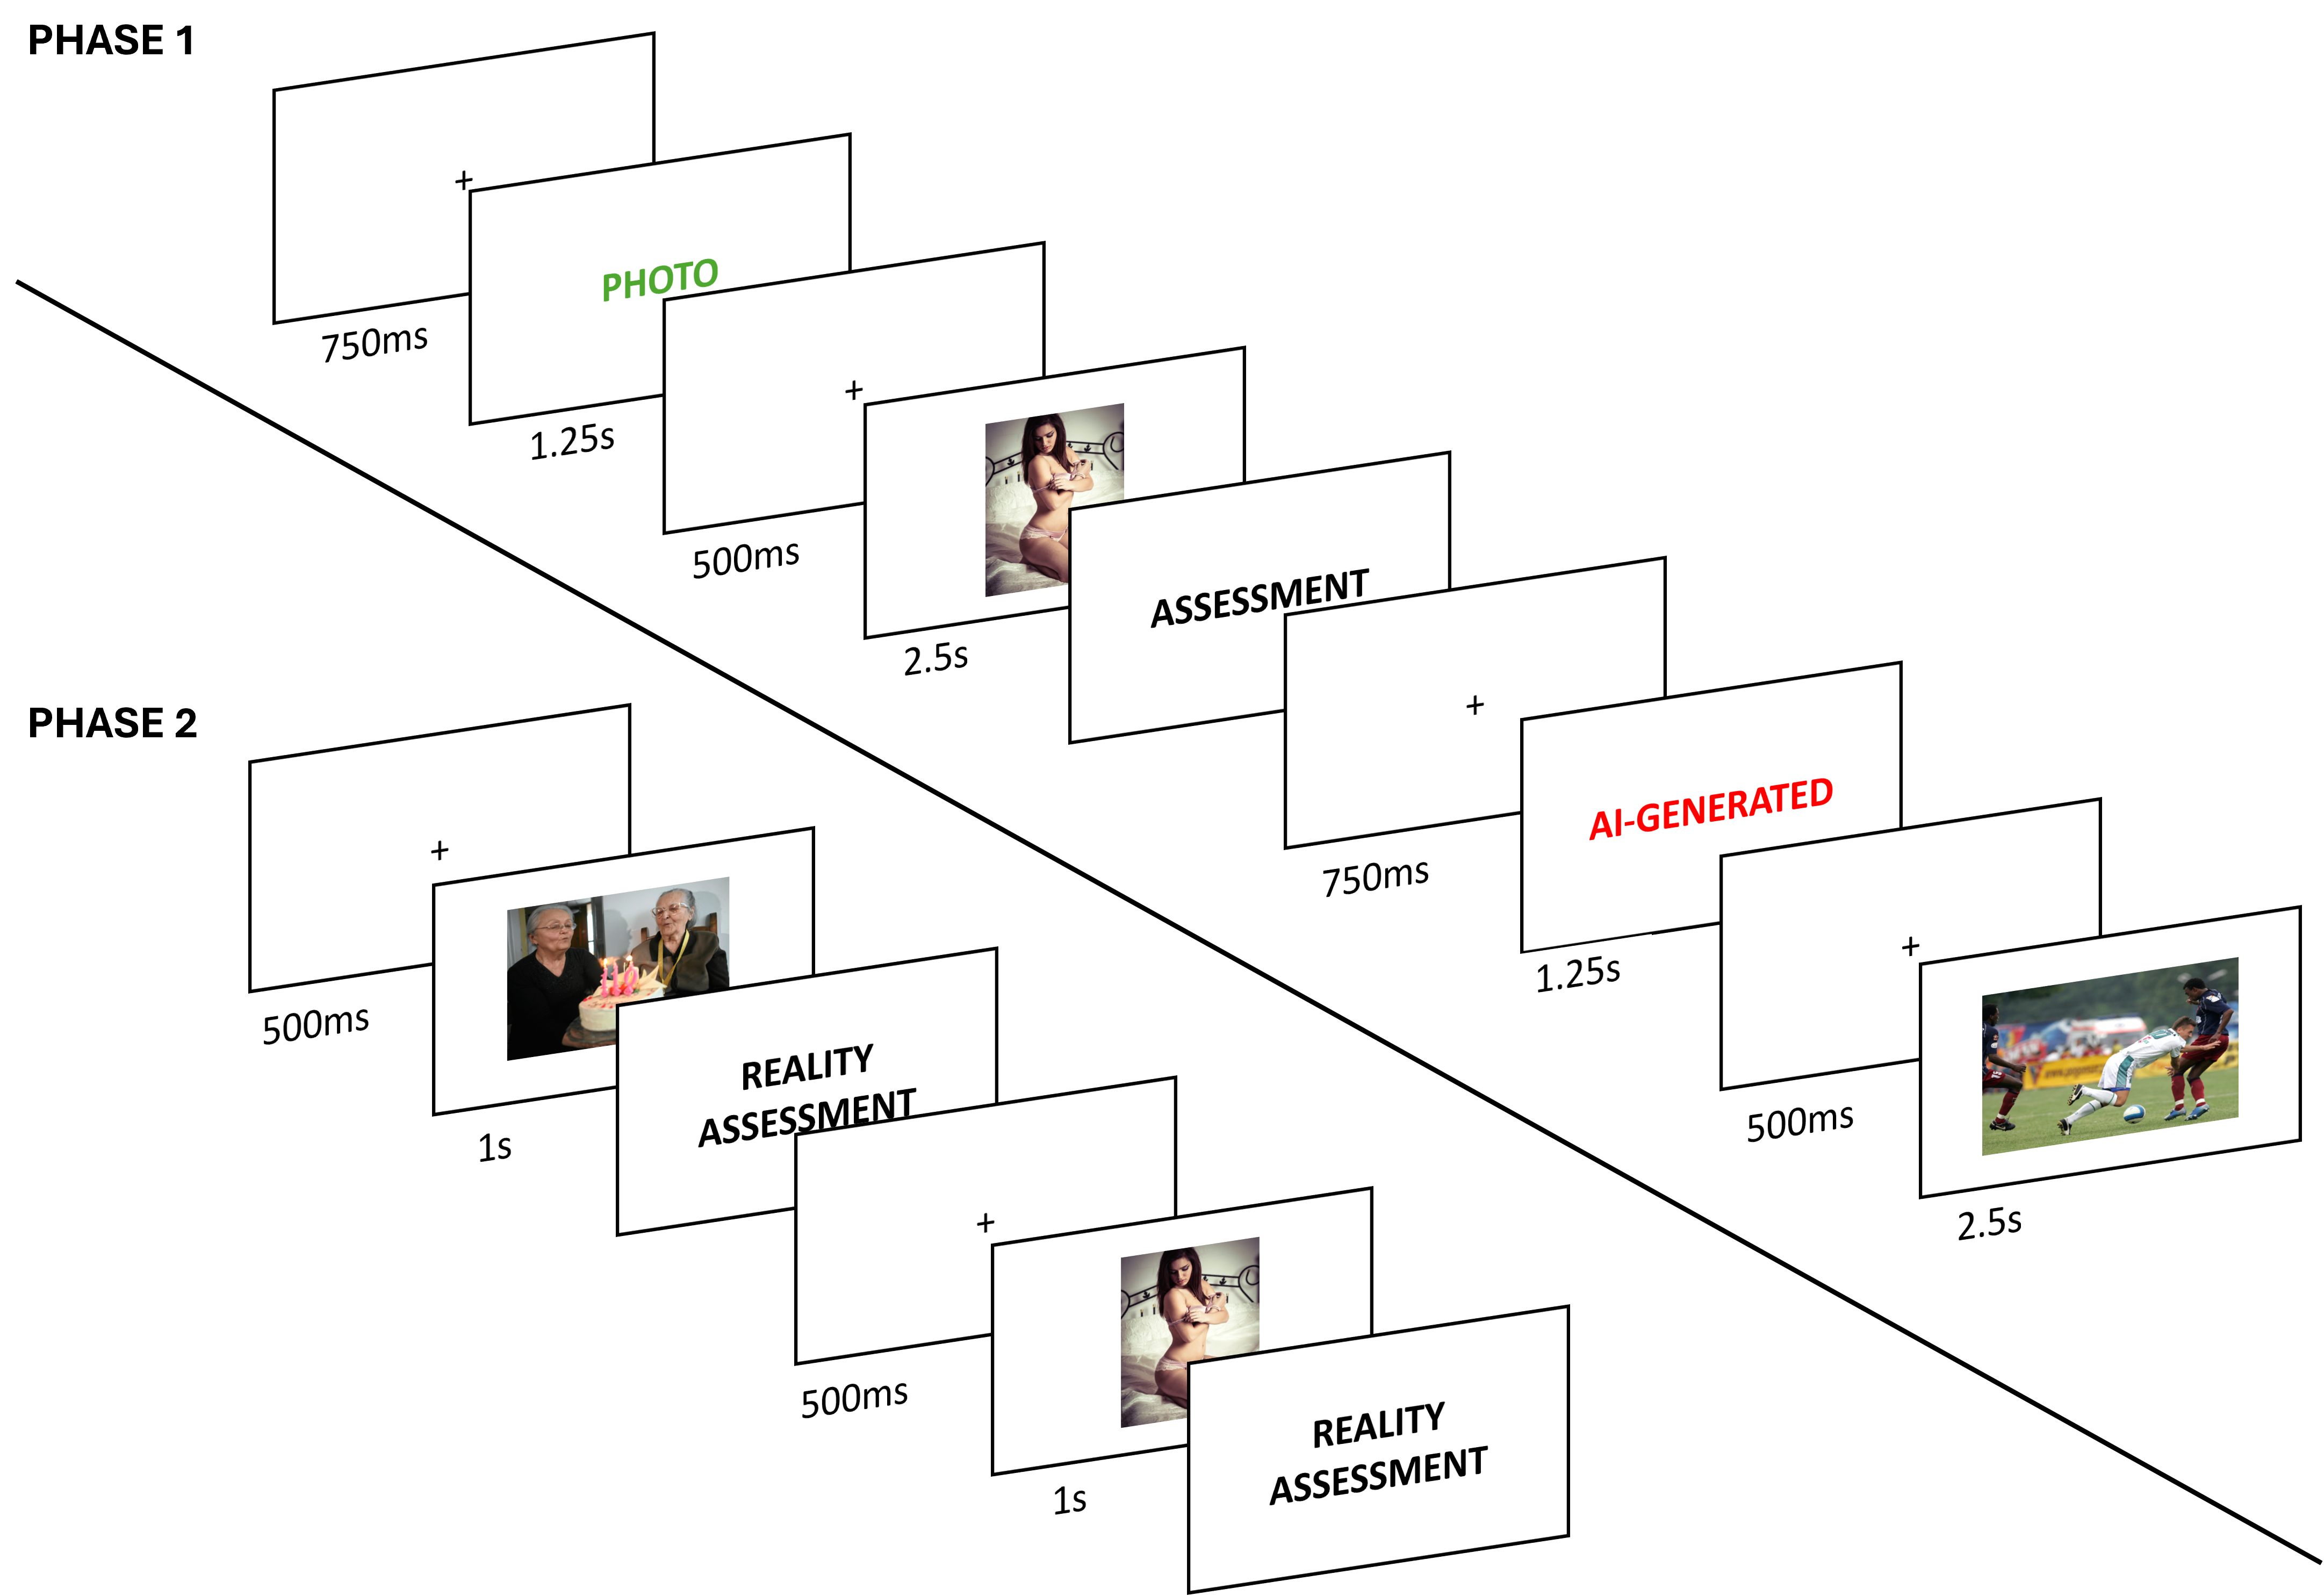
\includegraphics[width=1\linewidth,height=\textheight,keepaspectratio]{images/Paradigm1.png}

\end{figure*}

The study was conducted in line with the born-open principle
(\citeproc{ref-de2024datapipe}{Leeuw, 2024}), ensuring transparency and
reproducibility at every stage. The experiment was implemented entirely
in jsPsych (\citeproc{ref-de2015jspsych}{De Leeuw, 2015}), with the full
code hosted publicly on GitHub, which also served as the platform for
running the online study. Raw data were automatically stored in a
private Open Science Framework (OSF) repository. Anonymized data,
together with all preprocessing and analysis scripts, will be openly
released on GitHub to facilitate complete reproducibility. Participants
first provided informed consent before completing a short demographic
questionnaire covering gender, age, ethnicity, country of residence,
education, and English proficiency. Optional questions on birth control
use were also included. They then proceeded to the experimental tasks.

In the first phase, participants were told that the study aimed to
validate a new image-generation algorithm. They were informed that they
would see images allegedly produced by this algorithm intermixed with
real photographs, each preceded by a cue indicating whether the upcoming
image was of an ``AI-generated'' or ``Photograph'' origin. Their task
was to rate each image on arousal, enticement, and valence. Each
participant viewed 60 images in total: 40 erotic images (20 male and 20
female) from the Erotic subset of the Nencki Affective Picture System
(NAPS ERO, \citeproc{ref-wierzba2015erotic}{Wierzba et al., 2015}), and
20 additional images (10 neutral, 10 positively arousing) from the
original NAPS database (\citeproc{ref-marchewka2014nencki}{Marchewka et
al., 2014}). Each trial followed a fixed timing sequence: a fixation
cross (750 ms), a color-coded textual cue (1,250 ms), another fixation
cross (500 ms), then the image (2,500 ms). Cues were presented in red,
green, or blue, with colors randomly assigned across participants.

Following each image, participants rated their emotional response using
three continuous sliders assessing sexual arousal, enticement, and
valence. This phase was self-paced, with responses required before
continuing. After completing the image-rating phase, participants filled
out two self-report questionnaires: first the BAIT scale, followed by
the COPS questionnaire.

In the final phase, participants viewed the same 60 images, presented in
a new randomized order. Each was preceded by a 500 ms fixation cross and
displayed for 1,000 ms. This time, participants rated each image on
perceived realism---how photographic or lifelike it appeared.

At the end of the experiment, participants completed a feedback form.
They were asked whether they could distinguish AI-generated from real
images, whether AI images appeared more or less arousing, whether cue
labels seemed accurate or reversed, and whether specific images stood
out as particularly arousing or unarousing. Finally, participants were
debriefed on the true purpose of the study: to examine how image labels
(AI-generated vs.~real photograph) influence emotional responses.
Importantly, they were informed that all images were real photographs,
and that the ``AI-generated'' label was used solely to test the effect
of belief on affective reactions. A shareable link to the experiment was
also provided.

\textbf{Data Analysis}

\section{Study 2}\label{study-2}

\subsection{Methods}\label{methods-1}

\subsubsection{Participants}\label{participants}

The initial sample comprised 279 participants recruited via
Prolific\textcopyright. Inclusion criteria required participants to be
native English speakers or residents of countries with high levels of
English proficiency. Participant exclusions were applied as follows:
five participants were removed for showing no variability in arousal
ratings (i.e., they did not move the response scales). An additional
five participants were excluded for completing the study on a mobile
device. One participant was excluded due to displaying negative
correlations between arousal and both enticement and valence.
Furthermore, five participants who self-identified as neither female nor
male, and two participants who reported a sexual orientation other than
heterosexual, homosexual, or bisexual, were excluded from further
analyses. Finally, one participant was removed because the stimuli
presented were not relevant to their gender and sexual orientation.

The final sample consisted of 261 participants (Mean = 37.4 \(\pm\)
12.7, 48.7\% Female). 56.32\% of participants were from the United
Kingdom, 26.82\% from South Africa, 10.34\% from the United States, and
the remaining 6.51\% were from other countries.

Ethical approval for this study was obtained from the School of
Psychology Ethics Committee at the University of Sussex (ER/EB672/2).

\subsubsection{Materials}\label{materials-1}

\paragraph{Questionnaires.}\label{questionnaires-1}

The questionnaires used in Study 2 were largely the same as those in
Study 1, with minor modifications. In the BAIT, two items, assessing
beliefs that AI might take control of people and interest in using AI
systems in daily life, were removed. Additionally, the wording was
streamlined by replacing ``Artificial Intelligence'' with ``AI''
throughout the scale. In the COPS, the item assessing the typical
duration of pornography viewing sessions was omitted, retaining only
items measuring frequency of pornography viewing and recency of sexual
activity.

\paragraph{Affective Measures.}\label{affective-measures-1}

\paragraph{Arousal.}\label{arousal-1}

Subjective sexual arousal was assessed following each image with the
question, ``How much did you feel sexually aroused?'' Responses were
recorded on 6-point Likert scale from Not at all (0) to Very much (6).

\paragraph{Enticement.}\label{enticement-1}

Perceived enticement was measured after each image using the question,
``How enticing would you rate this image to be?'' with the same scale
ranging from 6-point Likert scale from Not at all (0) to Very much (6).

\paragraph{Valence.}\label{valence-1}

Emotional valence was evaluated by asking, ``The feeling evoked by the
image was\ldots{}'' rated on a scale from Unpleasant (0) to Pleasant
(6).

\paragraph{Reality.}\label{reality}

In a final stage of the experiment, each image was shown again, and
participants rated on the images authenticity with the question, ``I
think this face is\ldots Indicate your confidence that the image is fake
or real'' using a continuous scale anchored at AI-generated (-3) and
Photograph (3).

\paragraph{Feedback.}\label{feedback-1}

\subsubsection{Procedure}\label{procedure}

\begin{figure*}[!htbp]

{\caption{{Paradigm 2}{\label{fig-paradigm2}}}}

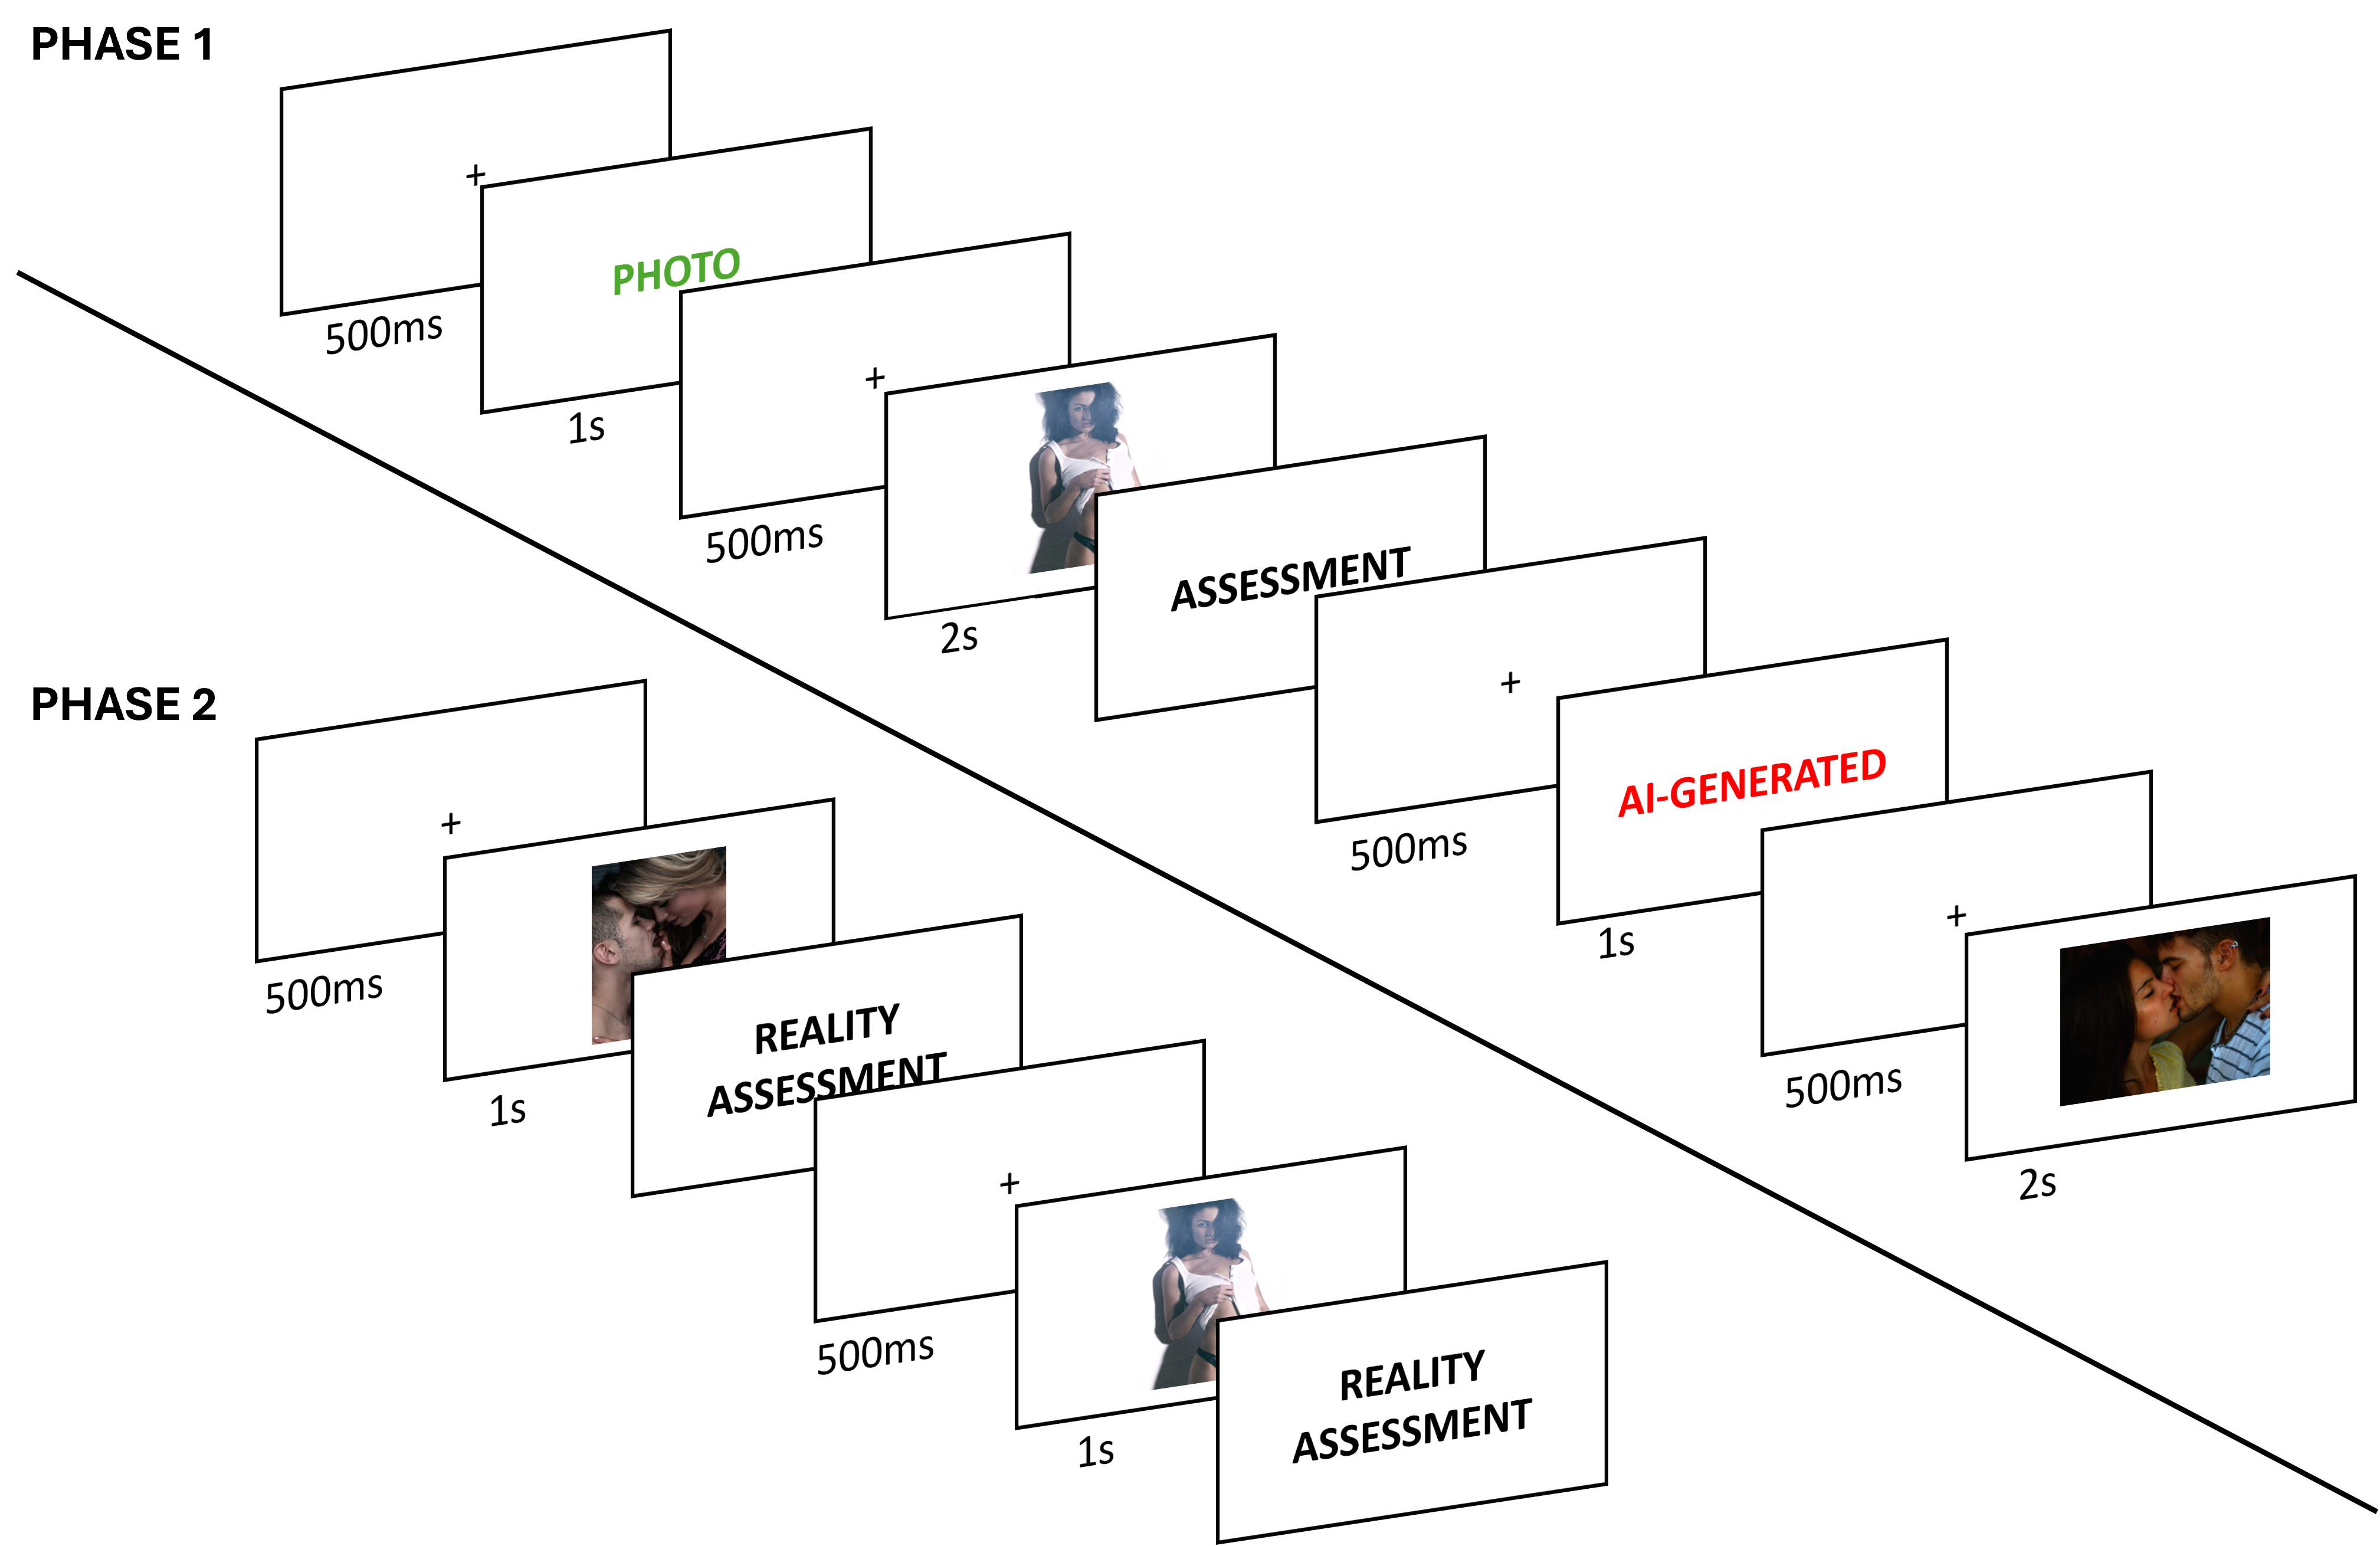
\includegraphics[width=1\linewidth,height=\textheight,keepaspectratio]{images/Paradigm2.png}

\end{figure*}

Consistent with Study 1, Study 2 was conducted in jsPsych following
born-open principles (\citeproc{ref-de2015jspsych}{De Leeuw, 2015};
\citeproc{ref-de2024datapipe}{Leeuw, 2024}).Participants first provided
informed consent, being informed that they could withdraw at any time;
however, once the experiment was completed, withdrawal was not possible
because the data were anonymized prior to storage. They then completed
the same demographic questions as in Study 1, with the exception of
items regarding birth control use.

In the first phase, participants were informed that the researchers were
collaborating with a young AI start-up based in Brighton, intended to
enhance the believability of the study. Participants were told that they
would view images generated by this algorithm intermixed with ``real''
photographs, each preceded by a label indicating whether the image was
AI-generated or a photograph. They were asked to rate each image on
sexual arousal, enticement, and valence. A total of 50 images were
presented, drawn from two categories of the NAPS-ERO database (25 images
of couples and 25 images of individuals).

Images were assigned to be relevant to participants' self-reported
gender and sexual orientation; for example, male participants
identifying as homosexual viewed male individuals and male couples. Each
trial followed a fixed timing sequence: a fixation cross (500 ms), a
color-coded textual cue displayed for 1,000 ms, a second fixation cross
(500 ms), and then the image presented for 2,000 ms. Cue colors were the
same as in Study 1 and were randomly assigned across trials.
Participants identifying as other in gender or bisexual/other in sexual
orientation were asked which type of images they preferred, with options
including ``Women (and heterosexual couples),'' ``Men (and heterosexual
couples),'' ``Only women (and lesbian couples),'' and ``Only men (and
gay couples).''

Midway through the 50 images, participants were provided with a break
and instructed to continue when ready. At this point, they completed a
brief feedback survey assessing their subjective impressions of the
images and AI-generation labels. This survey asked whether certain
images were particularly arousing, whether AI-generated images were more
or less arousing than the photographs, and participants' perceptions of
the AI-generation algorithm. Specifically, they indicated whether
differences between AI-generated and real images were obvious or subtle,
whether they perceived inconsistencies or reversals in labeling
(``Photograph'' vs.~``AI-Generated''), and whether they believed all
images were either photos or AI-generated. If participants indicated
that all images were real or AI-generated, they rated their confidence
on a scale from ``Not at all'' to ``Completely certain.'' This feedback
captured participants' explicit beliefs and subjective reactions
regarding both the content and labeling of the images.Following the
first phase, participants completed the BAIT and COPS questionnaires.

In the second phase, participants were informed that some images had
been intentionally mislabeled and were asked to judge whether each image
was AI-generated or a real photograph, expressing their confidence at
the extremes of the scale. The timing procedure in this phase was
identical to Study 1. After each image, participants provided general
feedback regarding their experience and any additional comments.
Finally, participants were presented with a debrief page informing them
that all images were, in fact, real photographs (see
Figure~\ref{fig-paradigm2}).

\subsubsection{Data Analysis}\label{data-analysis}

\section{References}\label{references}

\phantomsection\label{refs}
\begin{CSLReferences}{1}{0}
\bibitem[\citeproctext]{ref-corvi2023detection}
Corvi, R., Cozzolino, D., Zingarini, G., Poggi, G., Nagano, K., \&
Verdoliva, L. (2023). On the detection of synthetic images generated by
diffusion models. \emph{ICASSP 2023-2023 IEEE International Conference
on Acoustics, Speech and Signal Processing (ICASSP)}, 1--5.

\bibitem[\citeproctext]{ref-de2015jspsych}
De Leeuw, J. R. (2015). jsPsych: A JavaScript library for creating
behavioral experiments in a web browser. \emph{Behavior Research
Methods}, \emph{47}(1), 1--12.

\bibitem[\citeproctext]{ref-graber2021artificial}
Graber-Mitchell, N. (2021). \emph{Artificial illusions: Deepfakes as
speech}.

\bibitem[\citeproctext]{ref-hatch2023consumption}
Hatch, S. G., Esplin, C. R., Hatch, H. D., Halstead, A., Olsen, J., \&
Braithwaite, S. R. (2023). The consumption of pornography scale--general
(COPS--g). \emph{Sexual and Relationship Therapy}, \emph{38}(2),
194--218.

\bibitem[\citeproctext]{ref-kreps2022all}
Kreps, S., McCain, R. M., \& Brundage, M. (2022). All the news that's
fit to fabricate: AI-generated text as a tool of media misinformation.
\emph{Journal of Experimental Political Science}, \emph{9}(1), 104--117.

\bibitem[\citeproctext]{ref-de2024datapipe}
Leeuw, J. R. de. (2024). DataPipe: Born-open data collection for online
experiments. \emph{Behavior Research Methods}, \emph{56}(3), 2499--2506.

\bibitem[\citeproctext]{ref-marchewka2014nencki}
Marchewka, A., Żurawski, Ł., Jednoróg, K., \& Grabowska, A. (2014). The
nencki affective picture system (NAPS): Introduction to a novel,
standardized, wide-range, high-quality, realistic picture database.
\emph{Behavior Research Methods}, \emph{46}(2), 596--610.

\bibitem[\citeproctext]{ref-mcdonnell2010face}
McDonnell, R., \& Breidt, M. (2010). Face reality: Investigating the
uncanny valley for virtual faces. In \emph{ACM SIGGRAPH ASIA 2010
sketches} (pp. 1--2).

\bibitem[\citeproctext]{ref-meskys2020regulating}
Meskys, E., Kalpokiene, J., Jurcys, P., \& Liaudanskas, A. (2020).
Regulating deep fakes: Legal and ethical considerations. \emph{Journal
of Intellectual Property Law \& Practice}, \emph{15}(1), 24--31.

\bibitem[\citeproctext]{ref-miller2023ai}
Miller, E. J., Steward, B. A., Witkower, Z., Sutherland, C. A.,
Krumhuber, E. G., \& Dawel, A. (2023). AI hyperrealism: Why AI faces are
perceived as more real than human ones. \emph{Psychological Science},
\emph{34}(12), 1390--1403.

\bibitem[\citeproctext]{ref-nightingale2022ai}
Nightingale, S. J., \& Farid, H. (2022). AI-synthesized faces are
indistinguishable from real faces and more trustworthy.
\emph{Proceedings of the National Academy of Sciences}, \emph{119}(8),
e2120481119.

\bibitem[\citeproctext]{ref-schepman2020initial}
Schepman, A., \& Rodway, P. (2020). Initial validation of the general
attitudes towards artificial intelligence scale. \emph{Computers in
Human Behavior Reports}, \emph{1}, 100014.

\bibitem[\citeproctext]{ref-schepman2023general}
Schepman, A., \& Rodway, P. (2023). The general attitudes towards
artificial intelligence scale (GAAIS): Confirmatory validation and
associations with personality, corporate distrust, and general trust.
\emph{International Journal of Human--Computer Interaction},
\emph{39}(13), 2724--2741.

\bibitem[\citeproctext]{ref-wierzba2015erotic}
Wierzba, M., Riegel, M., Pucz, A., Leśniewska, Z., Dragan, W. Ł., Gola,
M., Jednoróg, K., \& Marchewka, A. (2015). Erotic subset for the nencki
affective picture system (NAPS ERO): Cross-sexual comparison study.
\emph{Frontiers in Psychology}, \emph{6}, 1336.

\end{CSLReferences}






\end{document}
